% !TEX root = ../main.tex
\iflatexml
\begin{figure}
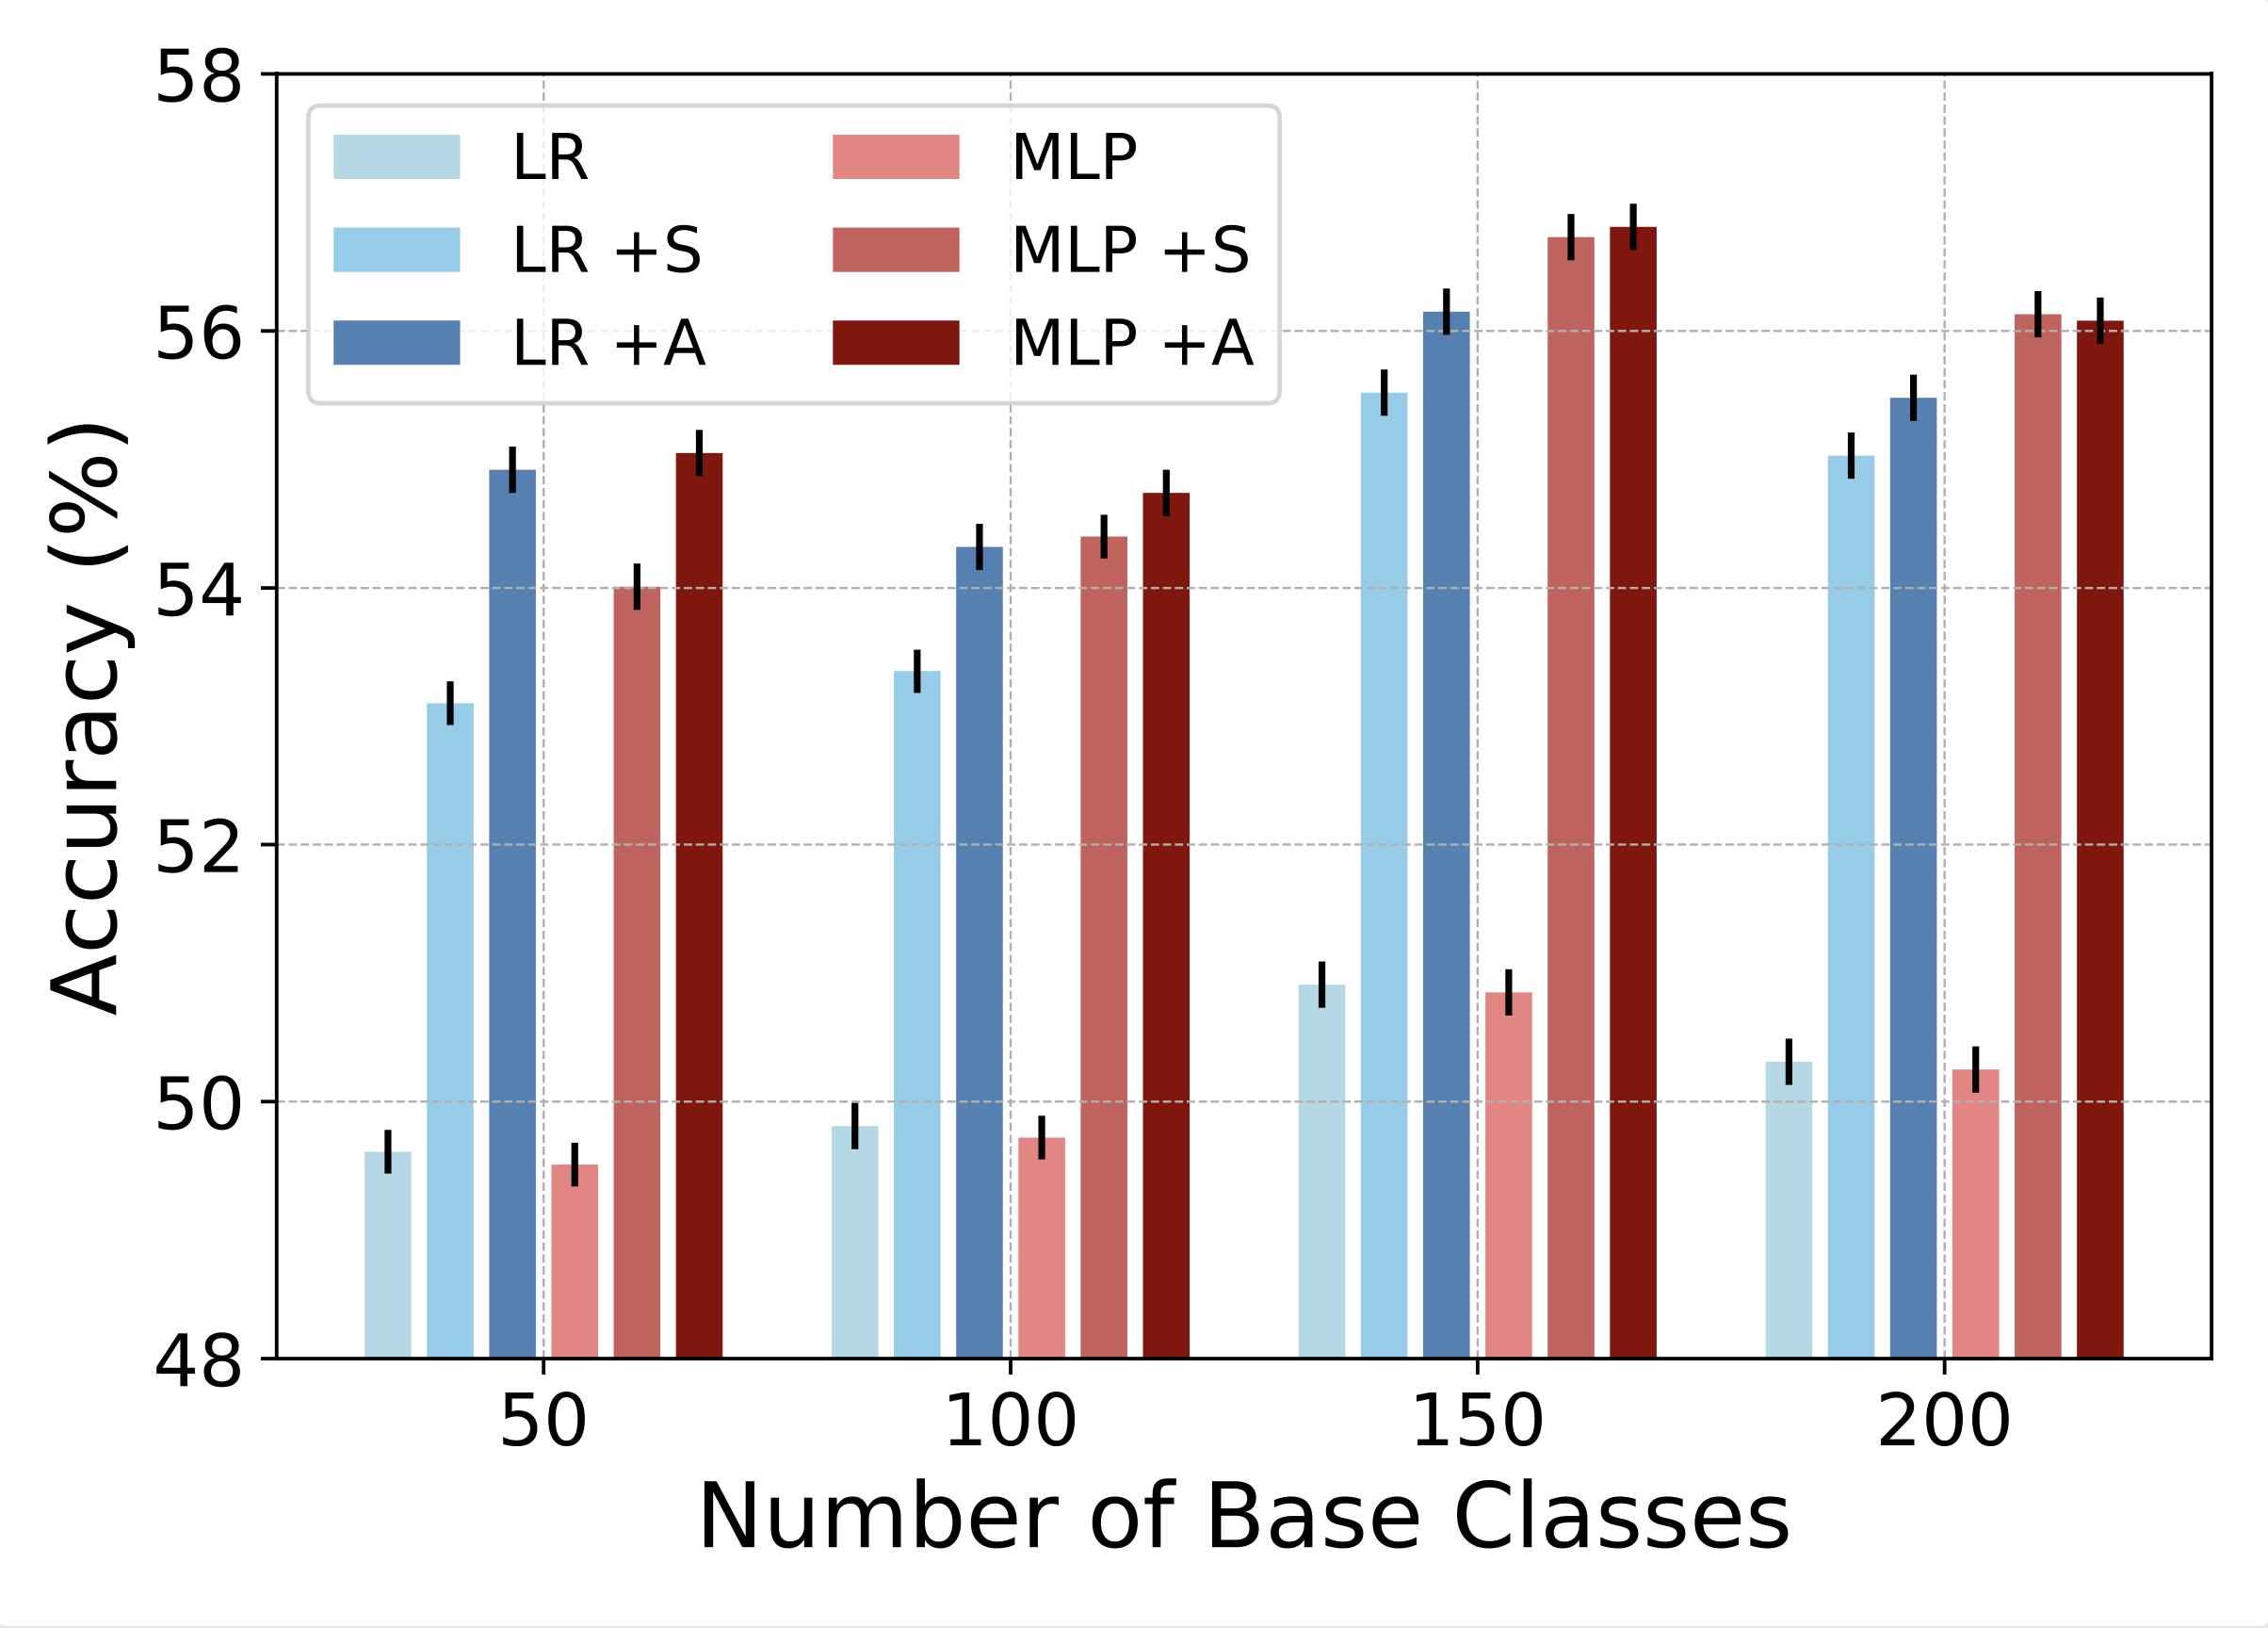
\includegraphics[width=4\textwidth]{figures/snapshot.png}
\caption{Results on \textit{tiered}-ImageNet with \{50, 100, 150, 200\} base classes.
\end{figure}
\else
\begin{wrapfigure}{R}{0.5\textwidth}
\vspace{-0.1in}
\centering
\hfill
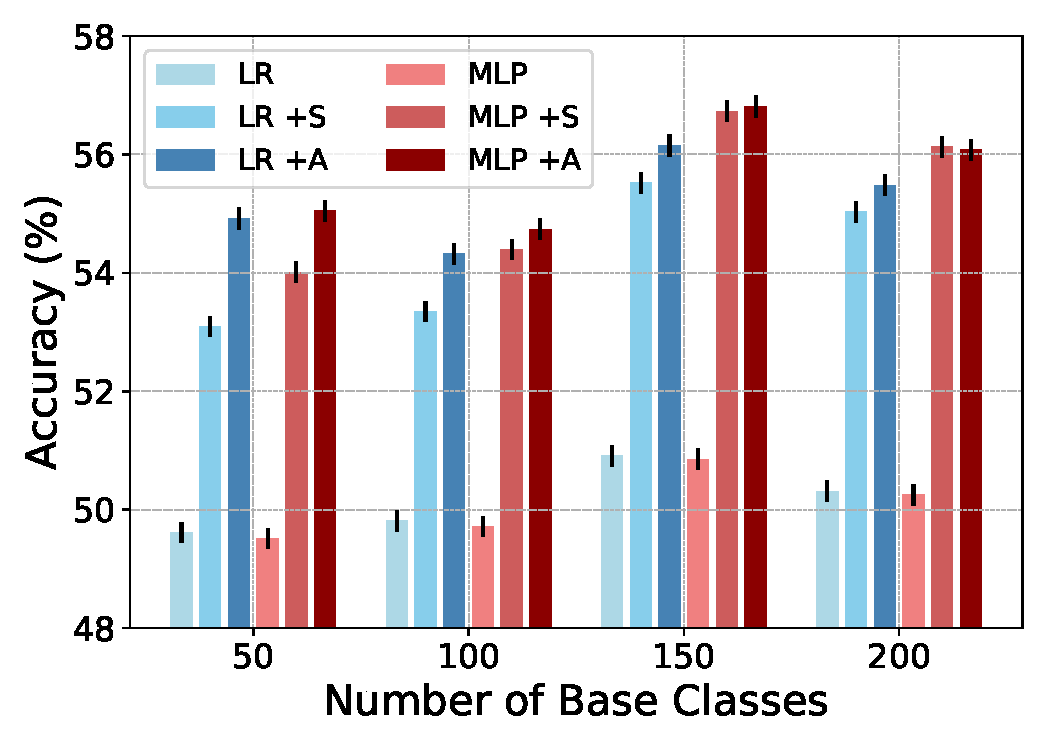
\includegraphics[width=0.5\textwidth,trim={0cm 0cm 0cm 0cm},clip]{figures/snapshot.pdf}
\caption{Results on \textit{tiered}-ImageNet with \{50, 100, 150, 200\} base classes.
}
\label{fig:snapshot}
\vspace{-0.25in}
\end{wrapfigure}
\fi